\newpage
\section{Introduction}
\label{sec:introduction}

\paragraph{} The main objective of this laboratory assignment is to study the circuit depicted in \ref{fig:circuit}. We decided to
separate this work in three different sections. \paragraph{}
In the first one,Theoretical Analysis \ref{sec:analysis}, we will analyze the circuit in 3 different
time intervals, $t<0$, $t=0$ and $t>0$. For the first 2 time intervals we will obtain linear equations using methods learnt in the TCFE class,
which can be solved with $Octave$. These equation allow to find the voltage in each node and the current
in each branch. With $t \rightarrow \infty $, a first order linear equation is obtained, which can be solved to obtain and plot the total solution of
the circuit. \paragraph{}
Using Ngspice tools, in the second section Simulation \ref{sec:simulation}, we will present a simulation of the circuit
and compare it with the previous theoretical results. \paragraph{}
Lastly, Conclusion \ref{sec:conclusion}, the contents of the report will be summarised and the achieved results discussed.

\begin{figure}[h]
    \centering
    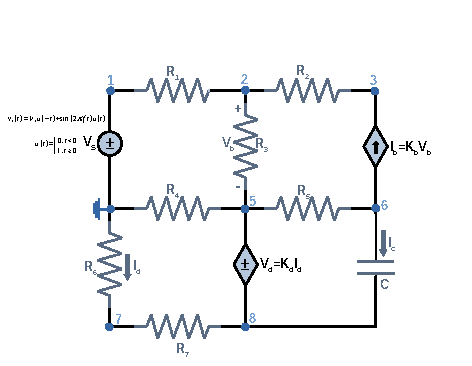
\includegraphics[width=0.8\linewidth]{circuit.pdf}
    \caption{Complet circuit}
    \label{fig:circuit}
\end{figure}

\begin{figure}[h]
    \centering
    \includegraphics[width=0.5\linewidth]{t4_incremental.pdf}
    \caption{Circuit for the op analysis}
    \label{fig:op_circuit}
\end{figure}

\begin{figure}[h]
    \centering
    \includegraphics[width=0.5\linewidth]{t4_opthevenin.pdf}
    \caption{Complet for the incremental analysis}
    \label{fig:inc_circuit}
\end{figure}

